\documentclass{article}
\usepackage[utf8]{inputenc}
\usepackage{float}
\usepackage{graphicx}
\usepackage{tabularx}
\usepackage{makecell}
\usepackage{fancyhdr}
\usepackage[round]{natbib}
\usepackage[english]{babel}
\usepackage[margin=1in]{geometry}
\usepackage{hyperref}
\usepackage{array, multirow}

\graphicspath{ {./images/SystemDesign} }

\pagestyle{fancy}  
\setlength\parindent{0pt}
\renewcommand\headrulewidth{0.4pt}                                      
\renewcommand\footrulewidth{0.4pt}

\title{SE 4GB6: Draft System Design\\The Cut}
\author{Group 17\\\\
            Joseph Lu - luy89 \\
            Matthew Po - pom \\
            Stanley Liu  liuz23 \\
            Suhavi Sandhu - sandhs11
            }
\date{\today}

% Setup fancyhdr package
\fancyhf{}
\fancyhfoffset{0em}
% Remove head rule
\renewcommand{\headrulewidth}{0pt}
\renewcommand{\footrulewidth}{0pt}
\fancyfoot[L]{Group17 - The Cut}
\fancyfoot[C]{Page \thepage}
\fancyfoot[R]{Revision 0}

\begin{document}

\maketitle
\newpage
\tableofcontents
\listoffigures
\listoftables
\newpage

\section{Revision}

\begin{table}[H]
    \caption{Revision}
    \centering
    \begin{tabularx}{\textwidth}{|c|c|c|X|}
        \hline
        Date & Revision Number & Authors & Comments \\ 
        \hline
        January 9, 2020 & 0 & \makecell{Matthew Po\\Suhavi Sandhu\\Stanley Liu\\Joseph Lu} & -\\ 
        \hline
    \end{tabularx}
    \label{tab:Revision}
\end{table}

\newpage

\section{Introduction}
 
\subsection{Project Purpose}
The purpose of this project is to create an Android application that identifies movies using videos recorded by the user. Currently, there exists no known off-the-shelf mobile application that can do this job. Much like popular mobile application, Shazam, which identifies songs based on audio, this application aims to fulfil a similar role for users who are having trouble identifying a movie.

\subsection{Document Purpose}
The purpose of this document is to decompose the application structure into components and give an overview of what each component does as well as how it relates to the requirements of the project.

\subsection{Scope}
The scope of the project is to be able to identify movies from short video clips. The development team will be focusing on Hollywood movies. Users will be able to input a video clip and the system will give a list of movies with confidence percentages. The scope of the information that will be retrieved is meta data such as actors, release date and description.

\subsection{Assumptions}

\begin{table}[H]
    \caption{Assumptions}
    \centering
    \begin{tabularx}{\textwidth}{|c|X|} \hline
        \textbf{A1} & The environment the user is in has a strong and stable network connection. \\ \hline
        Rationale & The application requires a steady connection to send large chunks of data such as video and will be inhibited if the connection is faulty.  \\ \hline \hline
        \textbf{A2} & The operating system which the application will run on is Android. \\ \hline
        Rationale & Development and testing will be focused to Android given prior experience of the team and budget constraints for developing on Android.  \\ \hline \hline
        \textbf{A3} & The user is an English speaker. \\ \hline
        Rationale & Support for languages outside of English is beyond the scope of the project. \\ \hline \hline
        \textbf{A4} & The video is recorded in a stable fashion and suitable lighting (no shaking and no dimly lit room). \\ \hline
        Rationale & Video stabilization and tweaking the brightness of the video post-recording is beyond the scope of the project. \\ \hline
    \end{tabularx}
    \label{tab:Assumptions}
\end{table}

\section{System Context}

\begin{figure}[H]
    \centering
    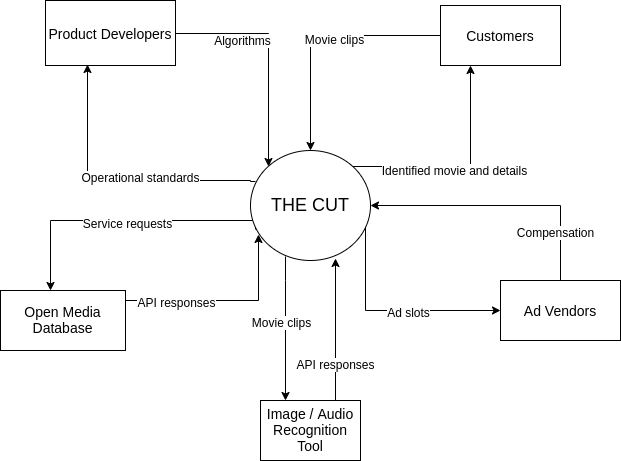
\includegraphics[width = \textwidth]{ContextDiagram.png}
    \caption{Context Diagram Showing Boundaries}
    \label{fig:Context}
\end{figure}

\section{Diagram of Components}

\begin{figure}[H]
    \centering
    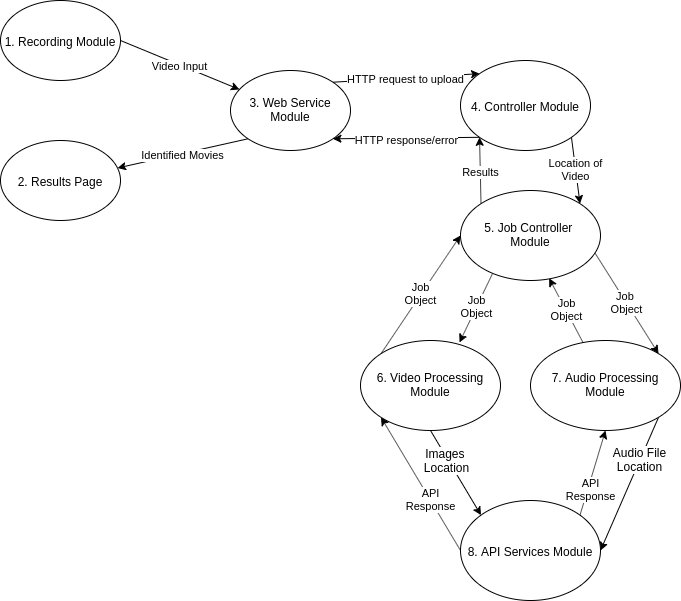
\includegraphics[width = \textwidth]{images/SystemDesign/ComponentDiagram.png}
    \caption{Diagram of Components}
    \label{fig:Component}
\end{figure}

\subsection{Anticipated Changes at Design Level}
\begin{enumerate}
    \item API services being used (currently Google Cloud Vision, imdb)
\end{enumerate}

\subsection{Unlikely Changes at Design Level}
\begin{enumerate}
    \item Operating System which will run the application (Android)
    \item Hardware which will run the application (Android smartphone)
    \item Implementation Language (JavaScript)
\end{enumerate}

\subsection{System Decomposition Tree}

\begin{figure}[H]
    \centering
    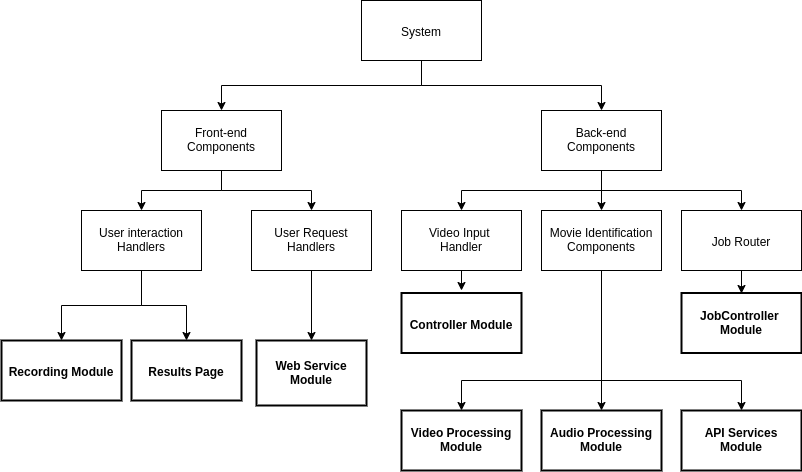
\includegraphics[width = \textwidth]{images/SystemDesign/system_decomp.png}
    \caption{System Decomposition Tree}
    \label{fig:Decomposition}
\end{figure}

\subsubsection{Hardware Hiding Modules}
\begin{enumerate}
    \item Recording Module
\end{enumerate}

\subsubsection{Behaviour Hiding Modules}
\begin{enumerate}
    \item Web Service Module
    \item Controller Module
    \item JobController
\end{enumerate}

\subsubsection{Software Hiding Modules}
\begin{enumerate}
    \item Results Page
    \item Video Processing Module
    \item Audio Processing Module
    \item API Services Module
\end{enumerate}

\subsection{Likelihood of Change}
\begin{table}[H]
    \caption{Likelihood of Change}
    \centering
    \begin{tabularx}{\textwidth}{|c|c|X|} \hline
        \textbf{Module} & \textbf{Likelihood of Change} & \textbf{Rationale} \\ \hline
         Recording Module & Very Unlikely & Key implementation aspect \\ \hline
         Results Page & Very Unlikely & Key implementation aspect \\ \hline
         Web Service Module & Very Unlikely & Key implementation aspect \\ \hline
         Controller Module & Very Unlikely & Key implementation aspect \\ \hline
         Job Controller Module & Very Unlikely & Key implementation aspect \\ \hline
         Video Processing Module & Very Unlikely & Key implementation aspect \\ \hline
         Audio Processing Module & Very Unlikely & Key implementation aspect \\ \hline
         API Service Module & Possible & Key implementation aspect \\ \hline
    \end{tabularx}
    \label{tab:likelihood of change}
\end{table}

\section{System Variables}

\subsection{Controlled and Monitored Variables}

\begin{table}[H]
    \caption{Variables}
    \centering
    \begin{tabularx}{\textwidth}{|c|X|c|c|c|}
        \hline
        \textbf{Name} & \textbf{Description} & \textbf{Type} & \textbf{Units} & \textbf{Range}\\
        \hline
        InputClipLength & Length of video submission & Monitored & Seconds & (10,60] \\
        \hline
    \end{tabularx}
    \label{tab:Variables}
\end{table}

\subsection{Constants}

\begin{table}[H]
    \caption{Constants}
    \centering
    \begin{tabularx}{\textwidth}{|c|X|c|c|}
        \hline
        \textbf{Name} & \textbf{Description} & \textbf{Units} & \textbf{Value}\\
        \hline
        $t_{MaxWaitTime}$ & Time constraint for application to respond to a request over a network. Should processing take longer than this (due to internet speed), the application will relinquish control back to the user and notify them once the results have been processed. & Seconds & 10 \\
        \hline
        $t_{MaxProcessingTime}$ & The maximum time it should take for video to be processed by both audio and image processing modules. Should processing take longer than the allotted time, it is considered to be failed. & Seconds & 120 \\
        \hline
        $MaxUploadAttempt$ & The max number of application attempts to upload a video file to the server. & Integer & 5 \\
        \hline
    \end{tabularx}
    \label{tab:Constants}
\end{table}

\section{Behaviour Overview}
The behaviour of each component is based on the secret it is trying to hide. 
\begin{enumerate}
    \item \textbf{Recording Module}: The user will interact with this module in order to record a video.
    \item \textbf{Results Page}: This page will fetch a list of which movies the user may have recorded.
    \item \textbf{Web Service Module}: This module will handle communication between the client and server side, such as uploading the video to a dedicated server space.
    \item \textbf{Controller Module}: This module will manage communication in the server and is responsible for sending errors and final results back to the user
    \item \textbf{JobController Module}: This module will route jobs to modules when necessary.
    \item \textbf{Video Processing Module}: This module will handle the way the visual portion of the input is analyzed.
    \item \textbf{Audio Processing Module}: This module will handle the way the auditory portion of the input is analyzed.
    \item \textbf{API Services Module}: This module will communicate with third-party APIs such as Google Cloud Vision.
\end{enumerate}

\section{Component Traceability}

\begin{table}[H]
    \caption{Recording Module Traceability}
    \centering
    \begin{tabular}{|l|c|} \hline
        \textbf{Component module} & \textbf{Functional and Non-Functional Requirements} \\ \hline
         \multirow{7}{*}{Recording Module} & F1 \\ \cline{2-2}
         & F2 \\ \cline{2-2}
         & NF1 \\ \cline{2-2}
         & NF2 \\ \cline{2-2}
         & NF4 \\ \cline{2-2}
         & NF8 \\ \cline{2-2}
         & NF12 \\ \hline
    \end{tabular}
    \label{tab:Recording_Traceability}
\end{table}

\begin{table}[H]
    \caption{Results Page Traceability}
    \centering
    \begin{tabular}{|l|c|} \hline
        \textbf{Component module} & \textbf{Functional and Non-Functional Requirements} \\ \hline
         \multirow{6}{*}{Results Page} & F3 \\ \cline{2-2}
         & F5 \\ \cline{2-2}
         & NF1 \\ \cline{2-2}
         & NF2 \\ \cline{2-2}
         & NF3 \\ \cline{2-2}
         & NF4 \\ \hline
    \end{tabular}
    \label{tab:Results_Traceability}
\end{table}

\begin{table}[H]
    \caption{Web Service Module Traceability}
    \centering
    \begin{tabular}{|l|c|} \hline
        \textbf{Component module} & \textbf{Functional and Non-Functional Requirements} \\ \hline
         \multirow{8}{*}{Web Service Module} & F4 \\ \cline{2-2}
         & F5 \\ \cline{2-2}
         & F6 \\ \cline{2-2}
         & NF5 \\ \cline{2-2}
         & NF9 \\ \cline{2-2}
         & NF10 \\ \cline{2-2}
         & NF11 \\ \cline{2-2}
         & NF12 \\ \hline
    \end{tabular}
    \label{tab:Web_Service_Traceability}
\end{table}

\begin{table}[H]
    \caption{Controller Module Traceability}
    \centering
    \begin{tabular}{|l|c|} \hline
        \textbf{Component module} & \textbf{Functional and Non-Functional Requirements} \\ \hline
         \multirow{4}{*}{Controller Module} & F3 \\ \cline{2-2}
         & F4 \\ \cline{2-2}
         & F5 \\ \cline{2-2}
         & NF6 \\ \hline
    \end{tabular}
    \label{tab:Controller_Traceability}
\end{table}

\begin{table}[H]
    \caption{Job Controller Module Traceability}
    \centering
    \begin{tabular}{|l|c|} \hline
        \textbf{Component module} & \textbf{Functional and Non-Functional Requirements} \\ \hline
         \multirow{3}{*}{Job Controller Module} & F3 \\ \cline{2-2}
         & F4 \\ \cline{2-2}
         & F5 \\ \hline
    \end{tabular}
    \label{tab:Job_Controller_Traceability}
\end{table}

\begin{table}[H]
    \caption{Video Processing Module Traceability}
    \centering
    \begin{tabular}{|l|c|} \hline
        \textbf{Component module} & \textbf{Functional and Non-Functional Requirements} \\ \hline
         \multirow{3}{*}{Video Processing Module } & F3 \\ \cline{2-2}
         & F4 \\ \cline{2-2}
         & NF7 \\ \hline
    \end{tabular}
    \label{tab:Video_Processing_Module}
\end{table}

\begin{table}[H]
    \caption{Audio Processing Module Traceability}
    \centering
    \begin{tabular}{|l|c|} \hline
        \textbf{Component module} & \textbf{Functional and Non-Functional Requirements} \\ \hline
         \multirow{3}{*}{Audio Processing Module } & F3 \\ \cline{2-2}
         & F4 \\ \cline{2-2}
         & NF7 \\ \hline
    \end{tabular}
    \label{tab:Audio_Processing_Module}
\end{table}

\begin{table}[H]
    \caption{API Service Module Traceability}
    \centering
    \begin{tabular}{|l|c|} \hline
        \textbf{Component module} & \textbf{Functional and Non-Functional Requirements} \\ \hline
         \multirow{3}{*}{API Service Module} & F5 \\ \cline{2-2}
         & NF7 \\ \cline{2-2}
         & NF12 \\ \hline
    \end{tabular}
    \label{tab:API_Services_Module}
\end{table}


\section{Component Overview}

\subsection{Recording Module}
\subsubsection{Description}
This module is a client side component that serves as a tool for recording video to be sent to our web services module

\subsubsection{Input/Output}
\textbf{Input:} User Input from device camera.

\textbf{Output:}
\begin{table}[H]
    \caption{Recording Module Output}
    \centering
    \begin{tabularx}{0.7\textwidth}{|c|c|c|c|X|} \hline
        \textbf{Name} & \textbf{Type} & \textbf{Range} & \textbf{Unit} & \textbf{Comments} \\ \hline
        VideoRecording & MP4 & [10,60] & Seconds & \\ \hline
    \end{tabularx}
    \label{tab:Recording_Output}
\end{table}

\subsubsection{Exception Handling}
\begin{table}[H]
    \caption{Recording Module Exception Handling}
    \centering
    \begin{tabularx}{0.7\textwidth}{|c|c|c|X|} \hline
        \textbf{Name} & \textbf{Type} & \textbf{ExceptionName} & \textbf{Behavior} \\ \hline
        VideoRecording & MP4 & InvalidClipLength & Cliend-Side-Validation \\ \hline
    \end{tabularx}
    \label{tab:Recording_Exception}
\end{table}

\subsubsection{Timing Constraint}
The video clip is constrained between 10 to 60 seconds of recording.

\subsubsection{Initialization}
At startup this module will initialize the device’s camera and await user input to start recording.

\subsubsection{Secret}
How the application records video.

\subsection{Web Service Module}

\subsubsection{Description}
This module is a client-side component responsible for sending the video file via HTTP Request for processing and analysis. It is also acts as a gateway for receiving results from the web server.

\subsubsection{Input/Output}
\textbf{Input:}
\begin{table}[H]
    \caption{Web Service Module Input}
    \centering
    \begin{tabularx}{0.7\textwidth}{|c|c|c|c|X|} \hline
        \textbf{Name} & \textbf{Type} & \textbf{Range} & \textbf{Unit} & \textbf{Comments} \\ \hline
        VideoRecording & MP4 & [10,60] & Seconds & Received from the RecordingModule\\ \hline
        AnalysisReport & JSON & & & \\ \hline
    \end{tabularx}
    \label{tab:Web_Service_Input}
\end{table}

\textbf{Output:}
\begin{table}[H]
    \centering
    \begin{tabularx}{0.7\textwidth}{|c|c|c|c|X|} \hline
        \textbf{Name} & \textbf{Type} & \textbf{Range} & \textbf{Unit} & \textbf{Comments} \\ \hline
        HttpRequest & JSON & & &\\ \hline
    \end{tabularx}
    \caption{Web Service Module Output}
    \label{tab:Web_Service_Output}
\end{table}

\subsubsection{Exception Handling}
\begin{table}[H]
    \caption{Web Service Exception Handling}
    \centering
    \begin{tabularx}{0.7\textwidth}{|c|c|c|X|} \hline
        \textbf{Name} & \textbf{Type} & \textbf{ExceptionName} & \textbf{Behavior} \\ \hline
        HttpRequest & JSON & BadRequest & Retry until 5 attempts reached \\ \hline
    \end{tabularx}
    \label{tab:Web_Service_Exception}
\end{table}

\subsubsection{Timing Constraint}
The time constraint of the HTTP Request and Response is defined by the (variable).

\subsubsection{Initialization}
This module awaits requests to send data to the server for processing.

\subsubsection{Secret}
How incoming requests are handled.

\subsection{JobController Module}

\subsubsection{Description}
This module is a server side component that is responsible for initializing and managing jobs to be run on the server. Each job corresponds to a video analysis request received by the Controller module. 

\subsubsection{Input/Output}
\textbf{Input:}
\begin{table}[H]
    \caption{JobController Input}
    \centering
    \begin{tabularx}{0.7\textwidth}{|c|c|c|c|X|} \hline
        \textbf{Name} & \textbf{Type} & \textbf{Range} & \textbf{Unit} & \textbf{Comments} \\ \hline
        VideoFileLocation & String & [1] & & Absolute path in server.\\ \hline
        PotentialMoviesIdentified & List<Object> & [0,100] & & \\ \hline
    \end{tabularx}
    \label{tab:JobController_Input}
\end{table}

\textbf{Output:}
\begin{table}[H]
    \caption{JobController Output}
    \centering
    \begin{tabularx}{0.7\textwidth}{|c|c|c|c|X|} \hline
        \textbf{Name} & \textbf{Type} & \textbf{Range} & \textbf{Unit} & \textbf{Comments} \\ \hline
        Results & JSON & [1] & & \\ \hline
        Job & Object & [1] & & \\ \hline
    \end{tabularx}
    \label{tab:JobController_Output}
\end{table}

\subsubsection{Exception Handling}
\begin{table}[H]
    \caption{JobController Exception Handling}
    \centering
    \begin{tabularx}{0.7\textwidth}{|c|c|c|X|} \hline
        \textbf{Name} & \textbf{Type} & \textbf{ExceptionName} & \textbf{Behavior} \\ \hline
        VideoFileLocation & String & InvalidFileLocation & Respond with a Job object with the failed state \\ \hline
    \end{tabularx}
    \label{tab:JobController_Exception}
\end{table}

\subsubsection{Timing Constraint}
Each job that is managed by this module will have a maximum allotted time of 120 seconds to identify the movie based on the video and audio modules. If it fails to do so, the job is timed out and is considered a fail. 

\subsubsection{Initialization}
This module awaits requests from the Controller module before initializing and managing jobs in the server.

\subsubsection{Secret}
How jobs in the server are managed.

\subsection{Video Processing Module}

\subsubsection{Description}

This module is a server-side component that is responsible for analyzing video data from a video file to determine what movie it is from with a high likelihood. It communicates with the APIService module to access services pertaining to the analysis of audio recordings.

\subsubsection{Input/Output}
\textbf{Input:}
\begin{table}[H]
    \caption{Video Processing Module Input}
    \centering
    \begin{tabularx}{0.7\textwidth}{|c|c|c|c|X|} \hline
        \textbf{Name} & \textbf{Type} & \textbf{Range} & \textbf{Unit} & \textbf{Comments} \\ \hline
        VideoFileLocation & String & [1] & Seconds & Absolute path in server \\ \hline
        APIResponse & Object & [1] & & \\ \hline
    \end{tabularx}
    \label{tab:Video_Processing_Input}
\end{table}

\textbf{Output:}
\begin{table}[H]
    \caption{Video Processing Module Output}
    \centering
    \begin{tabularx}{0.7\textwidth}{|c|c|c|c|X|} \hline
        \textbf{Name} & \textbf{Type} & \textbf{Range} & \textbf{Unit} & \textbf{Comments} \\ \hline
        PotentialMoviesIdentified & List<Object> & [0,100] & &\\ \hline
        ImagesLocation & String & [1] & & Absolute path in the server. \\ \hline
    \end{tabularx}
    \label{tab:Video_Processing_Output}
\end{table}

\subsubsection{Exception Handling}
\begin{table}[H]
    \caption{Video Processing Module Exception Handling}
    \centering
    \begin{tabularx}{0.7\textwidth}{|c|c|c|X|} \hline
        \textbf{Name} & \textbf{Type} & \textbf{ExceptionName} & \textbf{Behavior} \\ \hline
        APIResponse & JSON & BadServiceRequest & Return a failed result \\ \hline
    \end{tabularx}
    \label{tab:Video_Processing_Exception}
\end{table}

\subsubsection{Timing Constraint}
Timing constraints for this module are governed by the JobController time constraints. 

\subsubsection{Initialization}
This module awaits requests from Job objects before initializing and processing the data.

\subsubsection{Secret}
How the visual aspect of the video is processed.

\subsection{Audio Processing Module}

\subsubsection{Description}

This module is a server side component that is responsible for analyzing the audio data from a video file to determine the movie it is from with a high likelihood. It communicates with the APIService module to access services pertaining to the analysis of audio recordings.

\subsubsection{Input/Output}
\textbf{Input:}
\begin{table}[H]
    \caption{Audio Processing Module Input}
    \centering
    \begin{tabularx}{0.7\textwidth}{|c|c|c|c|X|} \hline
        \textbf{Name} & \textbf{Type} & \textbf{Range} & \textbf{Unit} & \textbf{Comments} \\ \hline
        VideoFileLocation & String & [1] & Seconds & Absolute path in server \\ \hline
        APIResponse & Object & [1] & & \\ \hline
    \end{tabularx}
    \label{tab:Audio_Processing_Input}
\end{table}

\textbf{Output:}
\begin{table}[H]
    \caption{Audio Processing Module Output}
    \centering
    \begin{tabularx}{0.7\textwidth}{|c|c|c|c|X|} \hline
        \textbf{Name} & \textbf{Type} & \textbf{Range} & \textbf{Unit} & \textbf{Comments} \\ \hline
        PotentialMoviesIdentified & List<Object> & [0,100] & &\\ \hline
        AudioFileLocation & String & [1] & & Absolute path in the server. \\ \hline
    \end{tabularx}
    \label{tab:Audio_Processing_Output}
\end{table}

\subsubsection{Exception Handling}
\begin{table}[H]
    \caption{Audio Processing Module Exception Handling}
    \centering
    \begin{tabularx}{0.7\textwidth}{|c|c|c|X|} \hline
        \textbf{Name} & \textbf{Type} & \textbf{ExceptionName} & \textbf{Behavior} \\ \hline
        APIResponse & JSON & BadServiceRequest & Return a failed result \\ \hline
    \end{tabularx}
    \label{tab:Audio_Processing_Exception}
\end{table}

\subsubsection{Timing Constraint}
Timing constraints for this module are governed by the JobController time constraints. 

\subsubsection{Initialization}
This module awaits requests from Job objects before initializing and processing the data.

\subsubsection{Secret}
How the audio aspect of the video is processed.

\subsection{API Service}

\subsubsection{Description}
This module is a server-side component that acts as a gateway to 3rd party APIs used by our application. It is responsible for handling all service requests by the Video and Audio modules.

\subsubsection{Input/Output}
\textbf{Input:}
\begin{table}[H]
    \caption{API Service Input}
    \centering
    \begin{tabularx}{0.7\textwidth}{|c|c|c|c|X|} \hline
        \textbf{Name} & \textbf{Type} & \textbf{Range} & \textbf{Unit} & \textbf{Comments} \\ \hline
        ImagesLocation & String & [1] & & Absolute path in the server. \\ \hline
        AudioFileLocation & String & [1] & & Absolute path in the server. \\ \hline
    \end{tabularx}
    \label{tab:API_Service_Input}
\end{table}

\textbf{Output:}
\begin{table}[H]
    \caption{API Service Output} 
    \centering
    \begin{tabularx}{0.7\textwidth}{|c|c|c|c|X|} \hline
        \textbf{Name} & \textbf{Type} & \textbf{Range} & \textbf{Unit} & \textbf{Comments} \\ \hline
        APIResponse & Object & [1] & & \\ \hline
    \end{tabularx}
    \label{tab:API_Service_Output}
\end{table}

\subsubsection{Exception Handling}
\begin{table}[H]
    \caption{API Service Exception Handling}
    \centering
    \begin{tabularx}{0.7\textwidth}{|c|c|c|X|} \hline
        \textbf{Name} & \textbf{Type} & \textbf{ExceptionName} & \textbf{Behavior} \\ \hline
        HttpRequest & JSON & BadRequest & Throw BadServiceRequest exception up the pipeline. \\ \hline
    \end{tabularx}
    \label{tab:API_Service_Exception}
\end{table}

\subsubsection{Timing Constraint}
Each API Request will have a timeout period during which it waits for the API to send a response. This timeout period is governed by the individual third-party API guidelines.

\subsubsection{Initialization}
This module awaits requests from the Video and Audio modules before initializing API Requests.

\subsubsection{Secret}
How the system gets information from third party APIs.

\subsection{Controller Module}

\subsubsection{Description}
This module is responsible for handling HTTP requests on the server. It also acts as a gateway for HTTP requests leaving the server. 

\subsubsection{Input/Output}
\textbf{Input:}
\begin{table}[H]
    \caption{Controller Module Input}
    \centering
    \begin{tabularx}{0.7\textwidth}{|c|c|c|c|X|} \hline
        \textbf{Name} & \textbf{Type} & \textbf{Range} & \textbf{Unit} & \textbf{Comments} \\ \hline
        HttpRequest & JSON & [1] & & \\ \hline
        Results & Object & [1] & & JobResults Object \\ \hline
    \end{tabularx}
    \label{tab:Controller_Input}
\end{table}

\textbf{Output:}
\begin{table}[H]
    \caption{Controller Module Output}
    \centering
    \begin{tabularx}{0.7\textwidth}{|c|c|c|c|X|} \hline
        \textbf{Name} & \textbf{Type} & \textbf{Range} & \textbf{Unit} & \textbf{Comments} \\ \hline
        VideoFileLocation & String & [1] & & Absolute path on the server \\ \hline
        Results & JSON & [1] & & \\ \hline
    \end{tabularx}
    \label{tab:Controller_Output}
\end{table}

\subsubsection{Exception Handling}
\begin{table}[H]
    \caption{Controller Module Exception Handling}
    \centering
    \begin{tabularx}{0.7\textwidth}{|c|c|c|X|} \hline
        \textbf{Name} & \textbf{Type} & \textbf{ExceptionName} & \textbf{Behavior} \\ \hline
        HttpRequest & JSON & BadRequest & \\ \hline
        VideoFileLocation & String & InvalidFileLocation & Delete the clip with the oldest timestamp not being used by a running job and retry to save the video file. \\ \hline
    \end{tabularx}
    \label{tab:Controller_Exception}
\end{table}

\subsubsection{Timing Constraint}
If the JobController does not alert the Controller module that a job has completed within 10 seconds, the Controller module alerts the client that the process is taking longer than usual and will send a follow up alert once the job has been completed.

\subsubsection{Initialization}
This module awaits HTTP Requests before calling for JobController to initialize a new job. It also waits for the JobController to alert it that a job has completed before sending the results to the client.

\subsubsection{Secret}
How the server processes HTTP requests and responses.

\subsection{Results Page Module}
\subsubsection{Description} 
This module is a client-side component that displays the results of the video analysis.

\subsubsection{Input/Output}
\textbf{Input:}
\begin{table}[H]
    \caption{Results Page Input}
    \centering
    \begin{tabularx}{0.7\textwidth}{|c|c|c|c|X|} \hline
        \textbf{Name} & \textbf{Type} & \textbf{Range} & \textbf{Unit} & \textbf{Comments} \\ \hline
        IdentifiedMovies & List<Object> & [0,100] & & \\ \hline
    \end{tabularx}
    \label{tab:Results_Page_Input}
\end{table}

\textbf{Output:} Android Native Application Page

\subsubsection{Exception Handling}
\begin{table}[H]
    \centering
    \begin{tabularx}{0.7\textwidth}{|c|c|c|X|} \hline
        \textbf{Name} & \textbf{Type} & \textbf{ExceptionName} & \textbf{Behavior} \\ \hline
        IdentifiedMovies & List<Object> & BadRequest & Redirect to the RecordVideo Module \\ \hline
    \end{tabularx}
    \caption{Results Page Exception Handling}
    \label{tab:Results_Page_Exception}
\end{table}

\subsubsection{Timing Constraint}
The screen shall display all relevant information within 3 seconds.

\subsubsection{Initialization}
This module is only display as a result of a video processing request made by recording a video in the RecordVideo module and sending a request to process.

\subsubsection{Secret}
How the plausible movies identified list is extracted and displayed.


\section{Normal Behaviour}
Under normal operating conditions, the application shall be able to run on a mobile device that supports Android 10 (https://developer.android.com/about/versions/10/features). The application shall have access to the mobile devices’ camera and microphone hardware to have the ability to take image, video, and/or audio snippets. The mobile device will be connected to the internet for quick results. 

\section{Undesired Event Handling}
\begin{enumerate}
    \item Application unexpectedly crashes during identification process/cell phone unexpectedly turns off
        \begin{itemize}
        \item The system will save the latest uploaded movie clip, so next time the user will not have to upload the clip again
        \item The system will automatically run a troubleshooting test to check the storage, memory usage, battery level the cell phone
        \end{itemize}
   \item Identification process takes too long due to weak internet signal or slow internet connection
        \begin{itemize}
        \item The system will notify the user about the internet latency and suggest the user to run the application under WIFI connection
        \end{itemize}
    \item Input clip length is too short to provide sufficient information for the application to identify the movie
        \begin{itemize}
        \item The system will notify the user to upload a longer clip, or film the video longer
        \end{itemize}
\end{enumerate}

\end{document}
